

\section{Experiments}


% \subsection{Implementation Details}
% We adopt Qwen2.5-VL-7B~\citep{bai2025qwen2} as the base model and apply the VeRL~\citep{sheng2024hybridflow} framework for reinforcement learning. Detailed implementation can be found in the Appendix.


\subsection{Implementation Details}

% We fine-tune Qwen2.5-VL-7B using GRPO under a distributed training setup based on DeepSpeed ZeRO-3. The model is trained on 8 A100 GPUs (80GB) using %DeepSpeed stage 3 with offloading disabled, and activation checkpointing enabled to reduce memory footprint. We use the AdamW optimizer with $(\beta_1 = %0.9, \beta_2 = 0.95)$ and weight decay set to 0.1. The learning rate is initialized at 5e-6 with a linear warmup of 500 steps followed by cosine decay. The %batch size per GPU is 1, resulting in an effective batch size of 8, and the maximum sequence length is set to 8192 tokens. Our final experimental results %were obtained after training for 3 days on 8 NVIDIA A100 GPUs.

We fine-tune the Qwen2.5-VL-7B model using GRPO within a distributed training setup based on Verl~\cite{sheng2024hybridflow, zheng2025easyr1}, utilizing 8 A100 GPUs (80GB). Throughout our experiments, we set the KL coefficient $ \beta= 1.0 \times 10^{-2} $. And for each problem instance, we sample 8 responses, each with a maximum length of 8192 tokens and a temperature of 1.0. Both the rollout batch size and the global batch size are set to 128. The actor model is updated using the AdamW optimizer with parameters $(\beta_1 = 0.9, \beta_2 = 0.99)$ and a learning rate $1.0 \times 10^{-6}$. The model is trained for 1.0 epoch for all experiments. Due to limited computational resources, we randomly sampled 43K documents from the 400K corpus for training. In our main results, we directly performed reinforcement learning on the base model using the 43K subset.



% \begin{table*}[t]
%   \begin{threeparttable}
%     \resizebox{1\textwidth}{!}{%
%       \begin{tabular}{l cc cc cc cc  cc | cc }
%       \toprule
%       \textbf{Methods}
%         & \multicolumn{2}{c|}{\textbf{Text\textsuperscript{Edit}}$\downarrow$} 
%         & \multicolumn{2}{c|}{\textbf{Form.\textsuperscript{Edit}}$\downarrow$} 
%         & \multicolumn{2}{c|}{\textbf{Table\textsuperscript{TEDS}}$\uparrow$} 
%         & \multicolumn{2}{c|}{\textbf{Table\textsuperscript{Edit}}$\downarrow$}
%         & \multicolumn{2}{c|}{\textbf{Read Order\textsuperscript{Edit}}$\downarrow$} 
%         & \multicolumn{2}{c}{\textbf{Overall\textsuperscript{Edit}}$\downarrow$} \\
%       \cmidrule{2-13}
%        & {\it EN} & {\it ZH} & {\it EN} & {\it ZH} 
%         & {\it EN} & {\it ZH} & {\it EN} & {\it ZH} 
%         & {\it EN} & {\it ZH} & {\it EN} & {\it ZH} \\
%       \midrule
%       \multicolumn{6}{l}{\textbf{Based on Pipeline Tools}} \\
    
%       MinerU~\citep{MinerU} 
%         & \textbf{0.061} & 0.215
%         & \textbf{0.278} & 0.577
%         & 78.6 & 62.1
%         &  0.18 & 0.344
%         & 0.079 & 0.292
%         & 0.15 & 0.357 \\
%       Marker~\citep{marker}
%         & 0.080 & 0.315
%         & 0.530 & 0.883
%         & 67.6 & 49.2
%         & 0.619 & 0.685
%         & 0.114 & 0.340
%         & 0.336 & 0.556 \\
%       Mathpix
%         & 0.105 & 0.384
%         & 0.306 & 0.454
%         & 77.0 & 67.1
%         & 0.243 & 0.320
%         & 0.108 & 0.304
%         & 0.191 & 0.365 \\
    
%     Docling~\citep{livathinos2025docling}
%         & 0.416 & 0.987
%         & 0.999 & 1.000
%         & 61.3 & 25.0
%         & 0.627 & 0.810
%         & 0.313 & 0.837
%         & 0.589 & 0.909 \\
%     Pix2Text~\citep{gurgurov2024image}
%         & 0.138 & 0.356
%         & 0.276 & 0.611
%         & 73.6 & 66.2
%         & 0.584 & 0.645
%         & 0.281 & 0.499
%         & 0.320 & 0.528 \\
%     Unstructured-0.17.2
%         & 0.198 & 0.481
%         & 0.999 & 1.000
%         & - & -
%         & 1.000 & 0.998
%         & 0.145 & 0.387
%         & 0.586 & 0.716 \\
%     OpenParse-0.7.0
%         & 0.681 & 0.974
%         & 0.996 & 1.000
%         & 64.8 & 27.5
%         & 0.284 & 0.639
%         & 0.595 & 0.641
%         & 0.646 & 0.814 \\
%     \midrule
%     \multicolumn{6}{l}{\textbf{Based on Expert VLMs}} \\
%       GOT-OCR~\citep{got2} 
%         & 0.189 & 0.315 & 0.360 & 0.528
%         & 53.2 & 47.2
%         & 0.459 & 0.520
%         & 0.141 & 0.280
%         & 0.287 & 0.411 \\
%       Nougat~\citep{Nougat} 
%         & 0.365 & 0.998 & 0.488 & 0.941
%         & 39.9 & 0.0
%         & 0.572 & 1.000
%         & 0.382 & 0.954
%         & 0.452 & 0.973 \\
%     Mistral OCR
%         & 0.072 & 0.325
%         & 0.318 & 0.495
%         & 75.8 & 63.6
%         & 0.600 & 0.650
%         & 0.083 & 0.284
%         & 0.268 & 0.439 \\
%     OLMOCR-sglang
%         & 0.097 & 0.293
%         & 0.455 & 0.655
%         & 68.1 & 61.3
%         & 0.608 & 0.652
%         & 0.145 & 0.277
%         & 0.326 & 0.469 \\
%     SmolDocling-256M
%         & 0.262 & 0.838
%         & 0.753 & 0.997
%         & 44.9 & 16.5
%         & 0.729 & 0.907
%         & 0.227 & 0.522
%         & 0.493 & 0.816 \\
        
%     \midrule
%     \multicolumn{6}{l}{\textbf{Based on General VLMs}} \\
%       GPT-4o~\citep{GPT4} 
%         & 0.144 & 0.409 & 0.425 & 0.606
%         & 72.0 & 62.9
%         & 0.234 & 0.329
%         & 0.128 & 0.251
%         & 0.233 & 0.399 \\
    
%     Qwen2-VL-72B~\citep{wang2024qwen2}   
%         & 0.096 & 0.218
%         & 0.404 & 0.487
%         & 76.8 & 76.4
%         & 0.387 & 0.408
%         & 0.119 & 0.193
%         & 0.252 & 0.327 \\
%     InternVL2-76B~\citep{InternVL}  
%         & 0.353 & 0.290
%         & 0.543 & 0.701
%         & 63.0 & 60.2
%         & 0.547 & 0.555
%         & 0.317 & 0.228
%         & 0.440 & 0.443 \\ 

%     Qwen2.5-VL-7B~\citep{bai2025qwen2.5}
%         & 0.142 & 0.205
%         & 0.393 & 0.530
%         & 78.7 & 78.3
%         & 0.155 & 0.162
%         & 0.191 & 0.169
%         & 0.220 & 0.265 \\
%     InternVL3-8B~\citep{zhu2025internvl3}
%         & 0.315 & 0.345
%         & 0.714 & 0.729
%         & 59.0 & 71.5
%         & 0.352 & 0.211
%         & 0.324 & 0.257
%         & 0.426 & 0.385 \\
%     \midrule
%     \multicolumn{6}{l}{\textbf{Based on Reinforcement Learning }} \\
%     Infinity-Parser-7B
%         & 0.076  & \textbf{0.117 }
%         & 0.314  & \textbf{0.434 }
%         & \textbf{85.3} & \textbf{81.4}
%         & \textbf{0.098} & \textbf{0.142}
%         & \textbf{0.076} & \textbf{0.095}
%         & \textbf{0.141} & \textbf{0.197} \\
%       \bottomrule
%       \end{tabular}%
%     }% end resizebox
%   \end{threeparttable}
%   \caption{Comprehensive evaluation of document parsing algorithms on OmniDocBench: performance metrics for text, formula, table, and reading order extraction, with overall scores derived from ground truth comparisons. }
%   \label{result_label1}
%   % \vspace{-2mm}
% \end{table*} 


% Gemini2.0-flash
    %     & 0.091 & 0.139
    %     & 0.389 & 0.584
    %     & 77.6 & 43.6
    %     & 79.7 & 78.9
    %     & 0.193 & 0.206
    %     & 0.092 & 0.128
    %     & 0.191 & 0.264 \\
    % Gemini2.5-Pro
    %     & \textbf{0.055} & 0.168
    %     & 0.356 & \textbf{0.439}
    %     & 80.0 & 69.4
    %     & \textbf{85.8} & \textbf{86.4}
    %     & \textbf{0.130} & \textbf{0.119}
    %     & \textbf{0.049} & \textbf{0.121}
    %      & \textbf{0.148} & \textbf{0.212} \\

    % \midrule
    % \multicolumn{6}{l}{\textit{Based on Open-Source  General VLMs}} \\


    


\begin{table*}[t]
  \begin{threeparttable}
    \resizebox{1\textwidth}{!}{%
      \begin{tabular}{l cc | cc  cc cc cc cc }
      \toprule
      \textbf{Methods}
        & \multicolumn{2}{c}{\textbf{Overall\textsuperscript{Edit}}$\downarrow$} 
        & \multicolumn{2}{c}{\textbf{Text\textsuperscript{Edit}}$\downarrow$} 
        & \multicolumn{2}{c}{\textbf{Form.\textsuperscript{Edit}}$\downarrow$} 
        & \multicolumn{2}{c}{\textbf{Table\textsuperscript{TEDS}}$\uparrow$} 
        & \multicolumn{2}{c}{\textbf{Table\textsuperscript{Edit}}$\downarrow$}
        & \multicolumn{2}{c}{\textbf{Read Order\textsuperscript{Edit}}$\downarrow$} \\
      \cmidrule{2-13}
       & {\it EN} & {\it ZH} 
       & {\it EN} & {\it ZH} 
       & {\it EN} & {\it ZH} 
       & {\it EN} & {\it ZH} 
       & {\it EN} & {\it ZH} 
       & {\it EN} & {\it ZH} \\
      \midrule
      \multicolumn{6}{l}{\textbf{Based on Pipeline Tools}} \\
    
      MinerU~\citep{MinerU} 
        & 0.15 & 0.357
        & \textbf{0.061} & 0.215
        & \textbf{0.278} & 0.577
        & 78.6 & 62.1
        &  0.18 & 0.344
        & 0.079 & 0.292 \\
      Marker~\citep{marker}
        & 0.336 & 0.556
        & 0.080 & 0.315
        & 0.530 & 0.883
        & 67.6 & 49.2
        & 0.619 & 0.685
        & 0.114 & 0.340 \\
      Mathpix
        & 0.191 & 0.365
        & 0.105 & 0.384
        & 0.306 & 0.454
        & 77.0 & 67.1
        & 0.243 & 0.320
        & 0.108 & 0.304 \\
    
    Docling~\citep{livathinos2025docling}
        & 0.589 & 0.909
        & 0.416 & 0.987
        & 0.999 & 1.000
        & 61.3 & 25.0
        & 0.627 & 0.810
        & 0.313 & 0.837 \\
    Pix2Text~\citep{gurgurov2024image}
        & 0.320 & 0.528
        & 0.138 & 0.356
        & 0.276 & 0.611
        & 73.6 & 66.2
        & 0.584 & 0.645
        & 0.281 & 0.499 \\
    Unstructured-0.17.2
        & 0.586 & 0.716
        & 0.198 & 0.481
        & 0.999 & 1.000
        & - & -
        & 1.000 & 0.998
        & 0.145 & 0.387 \\
    OpenParse-0.7.0
        & 0.646 & 0.814
        & 0.681 & 0.974
        & 0.996 & 1.000
        & 64.8 & 27.5
        & 0.284 & 0.639
        & 0.595 & 0.641 \\
    \midrule
    \multicolumn{6}{l}{\textbf{Based on Expert VLMs}} \\
      GOT-OCR~\citep{got2} 
        & 0.287 & 0.411
        & 0.189 & 0.315 
        & 0.360 & 0.528
        & 53.2 & 47.2
        & 0.459 & 0.520
        & 0.141 & 0.280 \\
      Nougat~\citep{Nougat} 
        & 0.452 & 0.973
        & 0.365 & 0.998 
        & 0.488 & 0.941
        & 39.9 & 0.0
        & 0.572 & 1.000
        & 0.382 & 0.954 \\
    Mistral OCR
        & 0.268 & 0.439
        & 0.072 & 0.325
        & 0.318 & 0.495
        & 75.8 & 63.6
        & 0.600 & 0.650
        & 0.083 & 0.284 \\
    OLMOCR-sglang
        & 0.326 & 0.469
        & 0.097 & 0.293
        & 0.455 & 0.655
        & 68.1 & 61.3
        & 0.608 & 0.652
        & 0.145 & 0.277 \\
    SmolDocling-256M
        & 0.493 & 0.816
        & 0.262 & 0.838
        & 0.753 & 0.997
        & 44.9 & 16.5
        & 0.729 & 0.907
        & 0.227 & 0.522 \\
        
    \midrule
    \multicolumn{6}{l}{\textbf{Based on General VLMs}} \\
      GPT-4o~\citep{GPT4} 
        & 0.233 & 0.399
        & 0.144 & 0.409
        & 0.425 & 0.606
        & 72.0 & 62.9
        & 0.234 & 0.329
        & 0.128 & 0.251 \\
    
    Qwen2-VL-72B~\citep{wang2024qwen2}   
        & 0.252 & 0.327
        & 0.096 & 0.218
        & 0.404 & 0.487
        & 76.8 & 76.4
        & 0.387 & 0.408
        & 0.119 & 0.193 \\
    InternVL2-76B~\citep{InternVL}  
        & 0.440 & 0.443
        & 0.353 & 0.290
        & 0.543 & 0.701
        & 63.0 & 60.2
        & 0.547 & 0.555
        & 0.317 & 0.228 \\ 

    Qwen2.5-VL-7B~\citep{bai2025qwen2.5}
        & 0.220 & 0.265
        & 0.142 & 0.205
        & 0.393 & 0.530
        & 78.7 & 78.3
        & 0.155 & 0.162
        & 0.191 & 0.169 \\
    InternVL3-8B~\citep{zhu2025internvl3}
        & 0.426 & 0.385
        & 0.315 & 0.345
        & 0.714 & 0.729
        & 59.0 & 71.5
        & 0.352 & 0.211
        & 0.324 & 0.257 \\
    \midrule
    \multicolumn{6}{l}{\textbf{Based on Reinforcement Learning }} \\
    Infinity-Parser-7B
        & \textbf{0.141} & \textbf{0.197} 
        & 0.076  & \textbf{0.117 }
        & 0.314  & \textbf{0.434 }
        & \textbf{85.3} & \textbf{81.4}
        & \textbf{0.098} & \textbf{0.142}
        & \textbf{0.076} & \textbf{0.095} \\
      \bottomrule
      \end{tabular}%
    }% end resizebox
  \end{threeparttable}
  \caption{Comprehensive evaluation of document parsing algorithms on OmniDocBench: performance metrics for text, formula, table, and reading order extraction, with overall scores derived from ground truth comparisons. }
  \label{result_label1}
  % \vspace{-3mm}
\end{table*}









\subsection{Main Results}


% \subsection{Evaluation and Metrics}
% In this section, we evaluate the model's performance in document parsing, table recognition, and Document-level OCR. In this work, 

We evaluate our method on several widely-used benchmarks for document understanding and OCR tasks. OmniDocBench~\citep{ouyang2024omnidocbench} provides comprehensive evaluation across diverse document types using NED and TEDS metrics. % Fox~\citep{liu2024focus_fox} offers multilingual assessment with 212 bilingual pages covering 9 sub-tasks. 
For table recognition, we use PubTabNet with scientific tables and FinTabNet~\citep{zheng2021global} with financial documents. Additionally, we employ olmOCR-Bench~\citep{poznanski2025olmocr} for fact-based OCR evaluation. We ensure that the test data for each benchmark undergoes rigorous text similarity filtering to prevent any overlap with the training data.  Detailed descriptions of these benchmarks are provided in Appendix. 


\paragraph{Overall Evaluation on OmniDocBench}
As shown in Table \ref{result_label1}, pipeline-based methods such as MinerU~\citep{MinerU} and Mathpix achieve superior performance across individual sub-tasks including text recognition and formula recognition. Meanwhile, general-purpose vision-language models like Qwen2.5-VL-7B and GPT-4o also demonstrate competitive results. Notably, most methods perform better on English pages compared to Chinese pages, reflecting language-dependent challenges. In contrast, our proposed Infinity-Parser-7B achieves a more balanced performance across all sub-tasks and languages, setting new SOTA results with overall edit distances of 0.141 and 0.197. This highlights the advantage of reinforcement learning with multi-aspect rewards in enabling robust, end-to-end document parsing.










 



% \begin{table}[h]
% \centering
% \resizebox{\linewidth}{!}{
% \begin{tabular}{lccccccccc}
% \toprule
% \textbf{Model} & \textbf{ArXiv} & \textbf{Old Scans Math} & \textbf{Tables} & \textbf{Old Scans} & \textbf{Headers\&Footers} & \textbf{Multi Col.} & \textbf{Long-Tiny Text} & \textbf{Base} & \textbf{Overall} \\
% \midrule
% GOT OCR & 52.7 & 52.0 & 0.2 & 22.1 & 93.6 & 42.0 & 29.9 & 94.0 & 48.3 \\
% Marker v1.6.2 & 24.3 & 22.1 & 69.8 & 24.3 & 87.1 & 71.0 & 76.9 & 99.5 & 59.4 \\
% MinerU v1.3.10 & 75.4 & 47.4 & 60.9 & 17.3 & \textbf{96.6} & 59.0 & 39.1 & 96.6 & 61.5 \\
% Mistral OCR API & 77.2 & 67.5 & 60.6 & 29.3 & 93.6 & 71.3 & 77.1 & 99.4 & 72.0 \\
% GPT-4o (No Anchor) & 51.5 & 75.5 & 69.1 & 40.9 & 94.2 & 68.9 & 54.1 & 96.7 & 68.9 \\
% GPT-4o (Anchored) & 53.5 & 74.5 & 70.0 & 40.7 & 93.8 & 69.3 & 60.6 & 96.8 & 69.9 \\
% Gemini Flash 2 (No Anchor) & 32.1 & 56.3 & 61.4 & 27.8 & 48.0 & 58.7 & 84.4 & 94.0 & 57.8 \\
% Gemini Flash 2 (Anchored) & 54.5 & 56.1 & 72.1 & 34.2 & 64.7 & 61.5 & 71.5 & 95.6 & 63.8 \\
% Qwen 2 VL (No Anchor) & 19.7 & 31.7 & 24.2 & 17.1 & 88.9 & 8.3 & 6.8 & 55.5 & 31.5 \\
% Qwen 2.5 VL (No Anchor) & 63.1 & 65.7 & 67.3 & 38.6 & 73.6 & 68.3 & 49.1 & 98.3 & 65.5 \\
% olmOCR v0.1.68 (No Anchor) & 72.1 & 74.7 & 71.5 & 43.7 & 91.6 & 78.5 & 80.5 & 98.1 & 76.3 \\
% olmOCR v0.1.68 (Anchored) & 75.6 & 75.1 & 70.2 & 44.5 & 93.4 & 79.4 & 81.7 & 99.0 & 77.4 \\
% \midrule
% Infinity-Parser-7B & \textbf{84.4} & \textbf{83.8} & \textbf{85.0} & \textbf{47.9} & 88.7 & \textbf{84.2} & \textbf{86.4} & \textbf{99.8} & \textbf{82.5} \\
% \bottomrule
% \end{tabular}
% }
% % \vspace{-1mm}
% % \caption{Performance comparison on the olmOCR~\citep{poznanski2025olmocr} benchmark across multiple document domains and structural challenges. Higher is better. Models labeled as No Anchor adopt an end-to-end parsing approach, relying solely on the visual input without any external metadata. In contrast, Anchor variants leverage additional structural hints extracted from PDF metadata using external parsers (e.g., layout coordinates), which serve as auxiliary signals to assist layout prediction.}
% \caption{Performance comparison on the olmOCR~\citep{poznanski2025olmocr} benchmark across multiple document domains and structural challenges. Higher is better.}
% \label{tab:olmocr_results}
% % \vspace{-3mm}
% \end{table}



\begin{table}[h]
\centering
\resizebox{\linewidth}{!}{
\begin{tabular}{l c|cccccccc}
\toprule
\textbf{Model} & \textbf{Overall} & \textbf{ArXiv} & \textbf{Old Scans Math} & \textbf{Tables} & \textbf{Old Scans} & \textbf{Headers\&Footers} & \textbf{Multi Col.} & \textbf{Long-Tiny Text} & \textbf{Base} \\
\midrule
GOT OCR & 48.3 & 52.7 & 52.0 & 0.2 & 22.1 & 93.6 & 42.0 & 29.9 & 94.0 \\
Marker v1.6.2 & 59.4 & 24.3 & 22.1 & 69.8 & 24.3 & 87.1 & 71.0 & 76.9 & 99.5 \\
MinerU v1.3.10 & 61.5 & 75.4 & 47.4 & 60.9 & 17.3 & \textbf{96.6} & 59.0 & 39.1 & 96.6 \\
Mistral OCR API & 72.0 & 77.2 & 67.5 & 60.6 & 29.3 & 93.6 & 71.3 & 77.1 & 99.4 \\
GPT-4o (No Anchor) & 68.9 & 51.5 & 75.5 & 69.1 & 40.9 & 94.2 & 68.9 & 54.1 & 96.7 \\
GPT-4o (Anchored) & 69.9 & 53.5 & 74.5 & 70.0 & 40.7 & 93.8 & 69.3 & 60.6 & 96.8 \\
Gemini Flash 2 (No Anchor) & 57.8 & 32.1 & 56.3 & 61.4 & 27.8 & 48.0 & 58.7 & 84.4 & 94.0 \\
Gemini Flash 2 (Anchored) & 63.8 & 54.5 & 56.1 & 72.1 & 34.2 & 64.7 & 61.5 & 71.5 & 95.6 \\
Qwen 2 VL (No Anchor) & 31.5 & 19.7 & 31.7 & 24.2 & 17.1 & 88.9 & 8.3 & 6.8 & 55.5 \\
Qwen 2.5 VL (No Anchor) & 65.5 & 63.1 & 65.7 & 67.3 & 38.6 & 73.6 & 68.3 & 49.1 & 98.3 \\
olmOCR v0.1.68 (No Anchor) & 76.3 & 72.1 & 74.7 & 71.5 & 43.7 & 91.6 & 78.5 & 80.5 & 98.1 \\
olmOCR v0.1.68 (Anchored) & 77.4 & 75.6 & 75.1 & 70.2 & 44.5 & 93.4 & 79.4 & 81.7 & 99.0 \\
\midrule
Infinity-Parser-7B & \textbf{82.5} & \textbf{84.4} & \textbf{83.8} & \textbf{85.0} & \textbf{47.9} & 88.7 & \textbf{84.2} & \textbf{86.4} & \textbf{99.8} \\
\bottomrule
\end{tabular}
}
\caption{Performance comparison on the olmOCR~\citep{poznanski2025olmocr} benchmark across multiple document domains and structural challenges. Higher is better.}
\label{tab:olmocr_results}
% \vspace{-5mm}
\end{table}







% \subsection{Document-Level OCR Evaluation on olmOCR-Bench}



\textbf{Document-level OCR Evaluation} Table \ref{tab:olmocr_results} reports performance on the olmOCR-Bench benchmark, which evaluates document-level OCR across diverse layouts and domains. Infinity-Parser-7B achieves the highest overall score (82.5), followed closely by olmOCR v0.1.68 (Anchored) (77.4), both demonstrating strong performance in complex categories like multi-column layouts and scanned math content. The results highlight the effectiveness of anchored prompting, with anchored versions of models (e.g., GPT-4o, olmOCR) significantly outperforming their non-anchored counterparts—especially on tables and old scans. This underscores the importance of layout-aware extraction techniques. In contrast, traditional pipelines like Marker and GOT OCR lag behind in structural accuracy, reinforcing the value of modern VLM-based approaches in high-fidelity PDF understanding.


\begin{table*}[h]
  % \centering
  \begin{minipage}[t]{0.47\textwidth}
    \vspace{0pt} % 对齐顶部
    % \small  
     \paragraph{Table Recognition Evaluation} To evaluate the model’s generalization ability, we introduce task-specific test cases. In Table~\ref{tab:teds_grouped_comparison}, we compare Infinity-Parser-7B with end-to-end table recognition models on PubTabNet and FinTabNet using the TEDS metric, which evaluates both structure and content. We also report TEDS-S for structure-only assessment. The evaluation results for InternVL3, Qwen2.5-VL, and GPT-4o were generated through our standardized benchmarking pipeline. Infinity-Parser-7B achieves the highest TEDS-S and TEDS scores on both datasets.
     % surpassing all baselines including strong models like InternVL3-78B and Qwen2.5-VL-72B.
  \end{minipage}
  \hfill
  \begin{minipage}[t]{0.5\textwidth}
    \vspace{0pt} % 对齐顶部
    \centering
    \small
    \renewcommand{\arraystretch}{1.1}
    \resizebox{\linewidth}{!}{%
    \begin{tabular}{lcccc}
      \toprule
      \textbf{Model} & \multicolumn{2}{c}{PubTabNet} & \multicolumn{2}{c}{FinTabNet} \\
      \cmidrule(lr){2-3} \cmidrule(lr){4-5}
      & TEDS-S & TEDS & TEDS-S & TEDS \\
      \midrule
      % EDD~\citep{zhong2020image} & 89.9 & 88.3 & 90.6 & - \\
      % OmniParser~\citep{wan2024omniparser} & 90.45 & 88.83 & 91.55 & 89.75 \\
      % InternVL3-8B~\citep{zhu2025internvl3} & 87.48 & 83.02 & 86.73 & 84.01 \\
      % InternVL3-78B~\citep{zhu2025internvl3} & 89.63 & 82.11 & 92.51 & 89.21 \\
      % Qwen2.5-VL-7B~\citep{bai2025qwen2} & 86.78 & 81.60 & 87.46 & 82.58 \\
      % Qwen2.5-VL-72B~\citep{bai2025qwen2} & 87.91 & 84.39 & 87.13 & 82.90 \\
      % GPT-4o~\citep{GPT4o} & 86.16 & 76.53 & 87.00 & 83.96 \\

      EDD & 89.9 & 88.3 & 90.6 & - \\
    OmniParser & 90.45 & 88.83 & 91.55 & 89.75 \\
    InternVL3-8B & 87.48 & 83.02 & 86.73 & 84.01 \\
    InternVL3-78B & 89.63 & 82.11 & 92.51 & 89.21 \\
    Qwen2.5-VL-7B & 86.78 & 81.60 & 87.46 & 82.58 \\
    Qwen2.5-VL-72B & 87.91 & 84.39 & 87.13 & 82.90 \\
    GPT-4o & 86.16 & 76.53 & 87.00 & 83.96 \\
      \midrule
      \textbf{Infinity-Parser-7B} & \textbf{93.46} & \textbf{91.82} & \textbf{97.16} & \textbf{95.92} \\
      \bottomrule
    \end{tabular}%
    }
    \captionof{table}{Comparisons of end-to-end table recognition methods on PubTabNet and FinTabNet.}
    \label{tab:teds_grouped_comparison}
  \end{minipage}
  % \vspace{-3mm}
\end{table*}






% \begin{table}[htbp]
%     \small
%     \centering
%     \renewcommand\arraystretch{1}
%     \setlength{\tabcolsep}{6pt}
%     \resizebox{1\linewidth}{!}{
%     \begin{tabular}{lccc cc|cc}
%         \toprule
%         \textbf{Method} & \textbf{Edit Dist. Reward} & \textbf{Count Reward} & \textbf{Order Reward} & \textbf{SFT} & \textbf{RL} & \textbf{Overall}\textsuperscript{Edit} $\downarrow$ & \textbf{Overall}\textsuperscript{Cat.} $\downarrow$ \\
%         \midrule
%         Zero Shot & - & - & - & -   & -    & 0.346 & 0.259 \\
%         SFT       & - & - & - & 27k & -    & 0.375 & 0.166 \\ 
%         \midrule
%         Zero + RL  & \CheckmarkBold & - & - & -   & 27k  & 0.287 & 0.156 \\
%         Zero + RL  & \CheckmarkBold & \CheckmarkBold & - & - & 27k & 0.280 & 0.141 \\
%         Zero + RL & \CheckmarkBold & \CheckmarkBold & \CheckmarkBold & - & 27k & 0.260 & 0.123 \\
%         \midrule
%         SFT + RL  & \CheckmarkBold & - & - & 300k  & 27k  & 0.345 & 0.244 \\
%         SFT + RL  & \CheckmarkBold & \CheckmarkBold & - & 300k  & 27k  & 0.345 & 0.244 \\
%         SFT + RL  & \CheckmarkBold & \CheckmarkBold & \CheckmarkBold & 300k  & 27k  & 0.345 & 0.244 \\
%         \bottomrule
%     \end{tabular}
%     }
%     \vspace{-2mm}
%     \caption{Results under different reward designs.}
%     \label{tab:test_rewards}
% \vspace{-3mm}
% \end{table}








\subsection{Ablation Study}

We perform ablation experiments to evaluate the individual contributions of our three core design choices: (1) data quality verification and (2) multi-aspect rewards. We report all ablation results using two primary evaluation metrics: Overall\textsuperscript{Edit} and Overall\textsuperscript{Cat.}. Overall\textsuperscript{Edit} represents the average edit-based overall score across English and Chinese pages, as shown in Table~\ref{result_label1}. In contrast, Overall\textsuperscript{Cat.} reflects the mean category-level performance across nine types of scanned document pages, following the same evaluation setting as Table 9 in the Appendix.  
% To save computational resources, the ablation studies are conducted on a randomly selected subset of 22K samples, rather than using the full 55K dataset as in the final results.


% \begin{table}[htbp]
%     \small
%     \centering
%     \renewcommand\arraystretch{1}
%     \setlength{\tabcolsep}{6pt}
%     \resizebox{1\linewidth}{!}{
%     \begin{tabular}{lccc cc|cc}
%         \toprule
%         \textbf{Method} & \textbf{Edit Dist. Reward} & \textbf{Count Reward} & \textbf{Order Reward} & \textbf{SFT} & \textbf{RL} & \textbf{Overall}\textsuperscript{Edit} $\downarrow$ & \textbf{Overall}\textsuperscript{Cat.} $\downarrow$ \\
%         \midrule
%         Zero Shot & - & - & - & -   & -    & 0.242 & 0.182 \\
%         SFT       & - & - & - & 43K & -    & 0.205 & 0.129 \\
%         SFT + RL  & - & - & - & 5k  & 37k  & 0.175 & 0.095 \\
%         Zero + RL  & \CheckmarkBold & - & - & -   & 43K  & 0.287 & 0.156 \\
%         Zero + RL  & \CheckmarkBold & \CheckmarkBold & - & - & 43K & 0.180 & 0.112 \\
%         Zero + RL & \CheckmarkBold & \CheckmarkBold & \CheckmarkBold & - & 43K & 0.169 & 0.106 \\
%         \bottomrule
%     \end{tabular}
%     }
%     % \vspace{-2mm}
%     \caption{Results under different reward designs.}
%     \label{tab:test_rewards}
% % \vspace{-3mm}
% \end{table}


\begin{table}[htbp]
    \small
    \centering
    \renewcommand\arraystretch{1}
    \setlength{\tabcolsep}{6pt}
    \resizebox{1\linewidth}{!}{
    \begin{tabular}{lccc cc|ccc}
        \toprule
        \textbf{Method} & \textbf{Edit Dist.} & \textbf{Count.} & \textbf{Order.} & \textbf{SFT} & \textbf{RL} & \textbf{Overall (EN)}\textsuperscript{Edit} $\downarrow$ & \textbf{Overall (ZH)}\textsuperscript{Edit} $\downarrow$ & \textbf{Overall }\textsuperscript{Cat.} $\downarrow$ \\
        \midrule
        Zero Shot & - & - & - & -   & -    & 0.220 & 0.265 & 0.183 \\
        SFT       & - & - & - & 43K & -    & 0.198 & 0.261 & 0.159 \\
        Zero + RL  & \CheckmarkBold & - & - & -   & 43K  & 0.169 & 0.224 & 0.156 \\
        Zero + RL  & \CheckmarkBold & \CheckmarkBold & - & - & 43K & 0.159 & 0.200 & 0.112 \\
        Zero + RL & \CheckmarkBold & \CheckmarkBold & \CheckmarkBold & - & 43K & 0.141 & 0.197 & 0.104 \\ 
        SFT + RL   & \CheckmarkBold & \CheckmarkBold & \CheckmarkBold & 43K & 43K    & 0.163 & 0.195 & 0.092 \\
        \bottomrule
    \end{tabular}
    } 
    \caption{Results under different reward designs.}
    \label{tab:test_rewards}
% \vspace{-5mm}
\end{table}


% \begin{table}[htbp]
%     \small
%     \centering
%     \renewcommand\arraystretch{1.1}
%     \setlength{\tabcolsep}{6pt}
%     \resizebox{1\linewidth}{!}{
%     \begin{tabular}{l|ccccc|cc|c}
%         \toprule
%         \multirow{2}{*}{\textbf{Method}} & \multicolumn{5}{c|}{\textbf{Reward Design}} & \multicolumn{3}{c}{\textbf{Evaluation Results}} \\
%         \cmidrule(lr){2-6} \cmidrule(lr){7-9}
%          & Edit & Count & Order & SFT Steps & RL Steps 
%          & OmniDoc (Edit) $\downarrow$ & OmniDoc (Cat.) $\downarrow$ & olmOCR $\downarrow$ \\
%         \midrule
%         Zero Shot   & - & - & - & -    & -    & 0.242 & 0.182 & 0.182 \\
%         SFT (55k)   & - & - & - & 55k  & -    & 0.205 & 0.129 & 0.129 \\
%         SFT (400k)  & - & - & - & 400k & -    & 0.191 & 0.101 & 0.101 \\
%         Zero + RL   & \CheckmarkBold & - & - & -    & 55k  & 0.287 & 0.156 & 0.156 \\
%         Zero + RL   & \CheckmarkBold & \CheckmarkBold & - & -    & 55k  & 0.180 & 0.112 & 0.112 \\
%         Zero + RL   & \CheckmarkBold & \CheckmarkBold & \CheckmarkBold & -    & 55k  & 0.169 & 0.106 & 0.106 \\
%         SFT + RL    & \CheckmarkBold & \CheckmarkBold & \CheckmarkBold & 400k & 55k  & 0.175 & 0.095 & 0.095 \\
%         \bottomrule
%     \end{tabular}
%     }
%     \caption{Results under different reward designs across OmniDoc and olmOCR benchmarks.}
%     \label{tab:test_rewards}
% \end{table}




% \textbf{Effect of Multi-Aspect Rewards.} Table~\ref{tab:test_rewards} shows that reinforcement learning consistently outperforms supervised fine-tuning, particularly under layout-aware reward designs. Compared to the SFT baseline (0.205 / 0.129), the RL method with distance-based reward (\textit{Zero + $R_{\text{dist}}$}) achieves better Overall\textsuperscript{Edit} (0.169) and comparable Overall\textsuperscript{Cat.} (0.156). Further introducing count and order rewards leads to significant improvements in structural consistency, with \textit{Zero + $R_{\text{dist}} + R_{\text{count}}$} achieving 0.280\textsuperscript{} / 0.141\textsuperscript{}, and the full reward setting reaching 0.260 / 0.123. These results highlight RL’s ability to incorporate structural inductive biases via reward design, enabling better alignment with task-specific goals and reducing overfitting to token-level patterns. The improvements across reward configurations confirm the effectiveness of multi-aspect rewards in enhancing layout-aware generalization.


\paragraph{Effect of Multi-Aspect Rewards.} Table~\ref{tab:test_rewards} demonstrates that reinforcement learning can outperform supervised fine-tuning when appropriate reward designs are applied. Compared to the SFT baseline (0.198 / 0.261 / 0.159), the RL method with distance-based reward (\textit{Zero + $R_{\text{dist}}$}) achieves better Overall\textsuperscript{Edit} (EN: 0.169 vs. 0.198, ZH: 0.224 vs. 0.261) while maintaining a comparable Overall\textsuperscript{Cat.} (0.156 vs. 0.159). Incorporating additional count and order rewards further improves structural consistency: \textit{Zero + $R_{\text{dist}} + R_{\text{count}}$} achieves 0.159 / 0.200 / 0.112, and \textit{Zero + $R_{\text{dist}} + R_{\text{count}} + R_{\text{order}}$} achieves 0.141 / 0.197 / 0.104. Meanwhile, when reinforcement learning is combined with supervised fine-tuning (\textit{SFT + RL}), the model does not exhibit further significant improvements. This observation is consistent with existing studies~\citep{guo2025deepseek}, which suggest that given the backbone model’s inherent capabilities, SFT may be unnecessary for downstream RL training in certain scenarios. These results further demonstrate that reinforcement learning, when equipped with structural supervisory signals, enables the model to better align with task-specific objectives.





\begin{figure}[h!]
    \centering
    % 子图1
    \begin{subfigure}{0.49\textwidth}
        \centering
        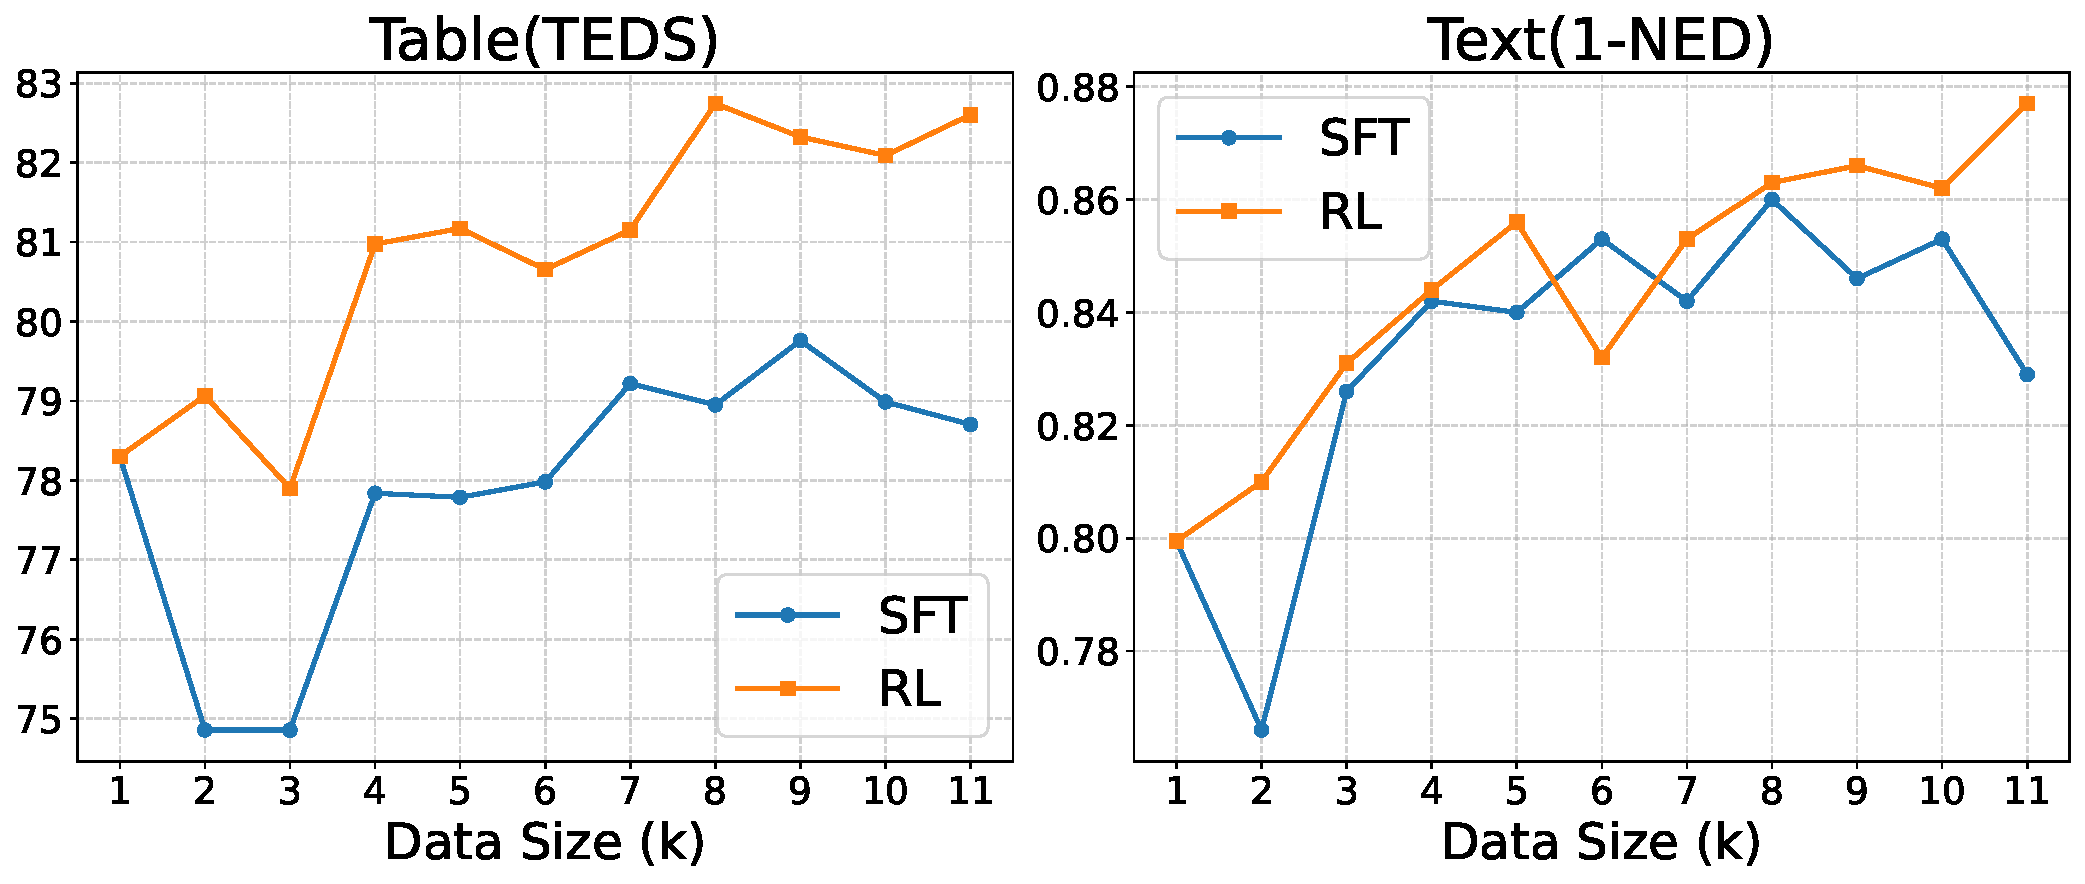
\includegraphics[width=\linewidth]{picture/metrics_pair1.pdf}
        % \vspace{-2mm}
        % \caption{In-Distribution Task}
        \label{fig:metrics_indist}
    \end{subfigure}
    % 子图2
    \begin{subfigure}{0.49\textwidth}
        \centering
        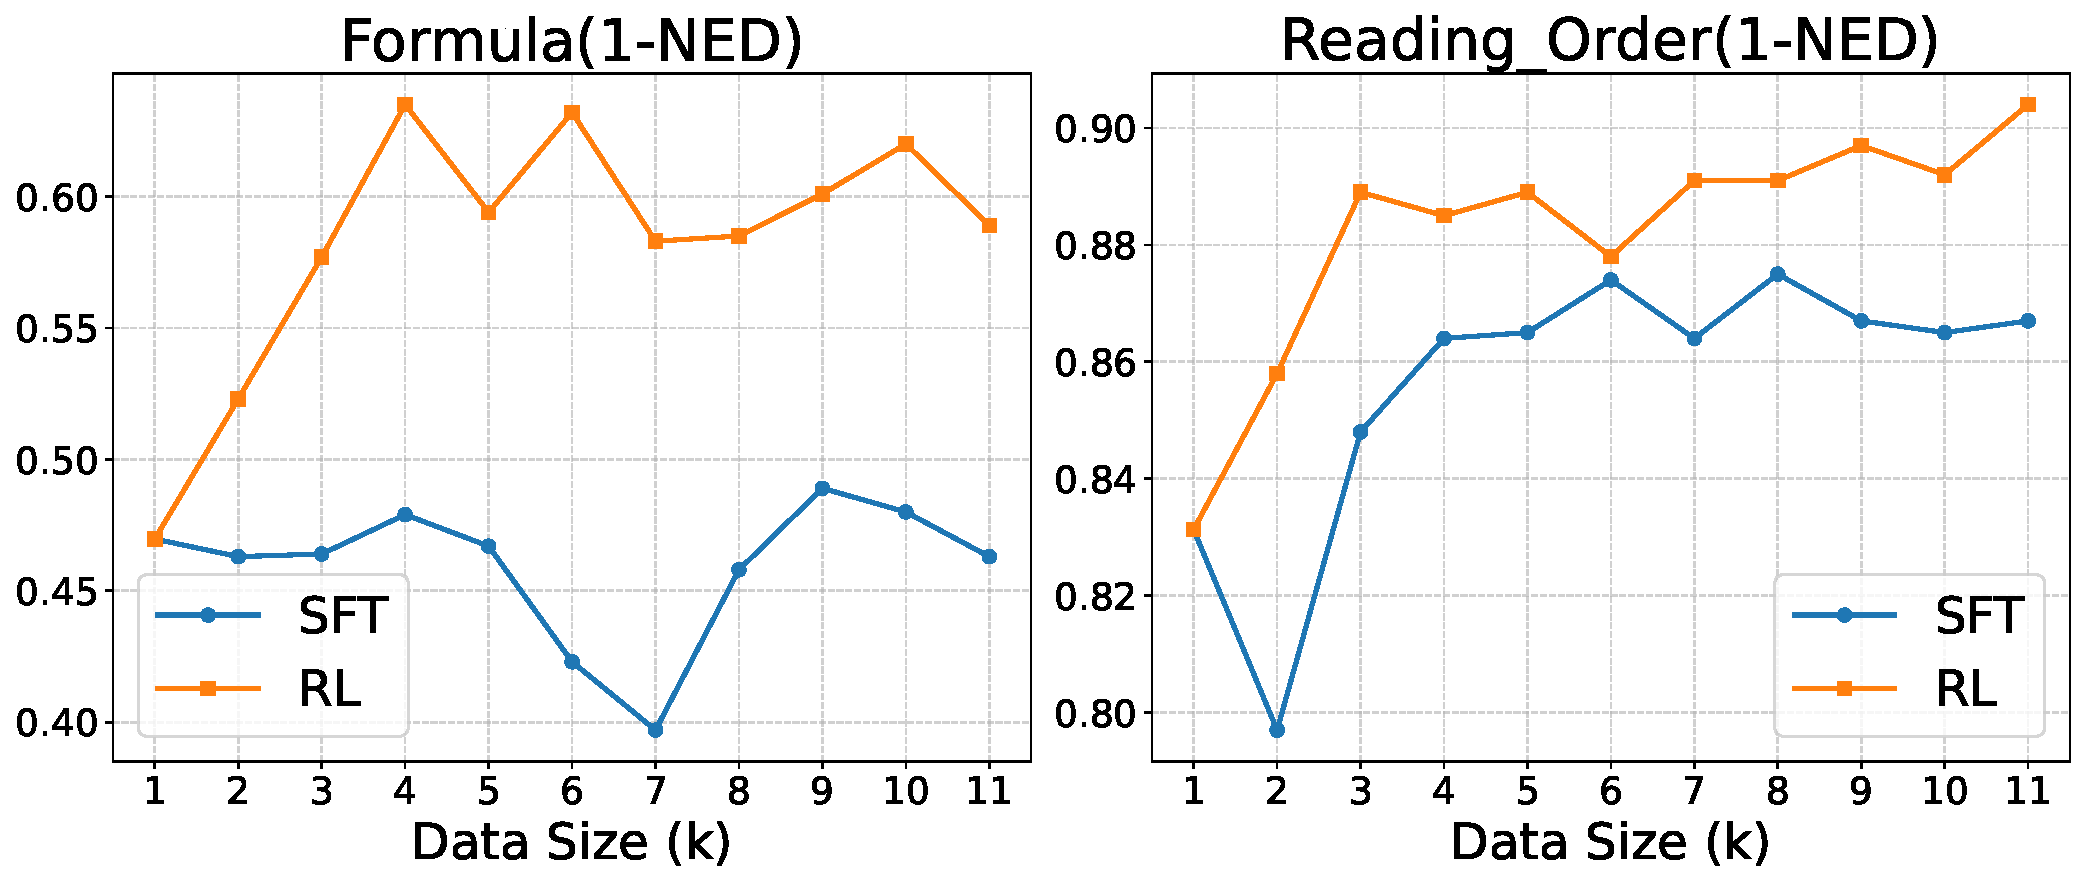
\includegraphics[width=\linewidth]{picture/metrics_pair2.pdf}
        % \vspace{-2mm}
        % \caption{Out-of-Distribution Task}
        \label{fig:metrics_ood}
    \end{subfigure}
    \vspace{-5mm}
    \caption{Performance comparison of SFT and Layout-Aware RL on OmniDocBench sub-tasks.}
    \label{fig:metrics_comparison}
    \vspace{-2mm}
\end{figure}

\begin{figure}[h!]
    \centering
    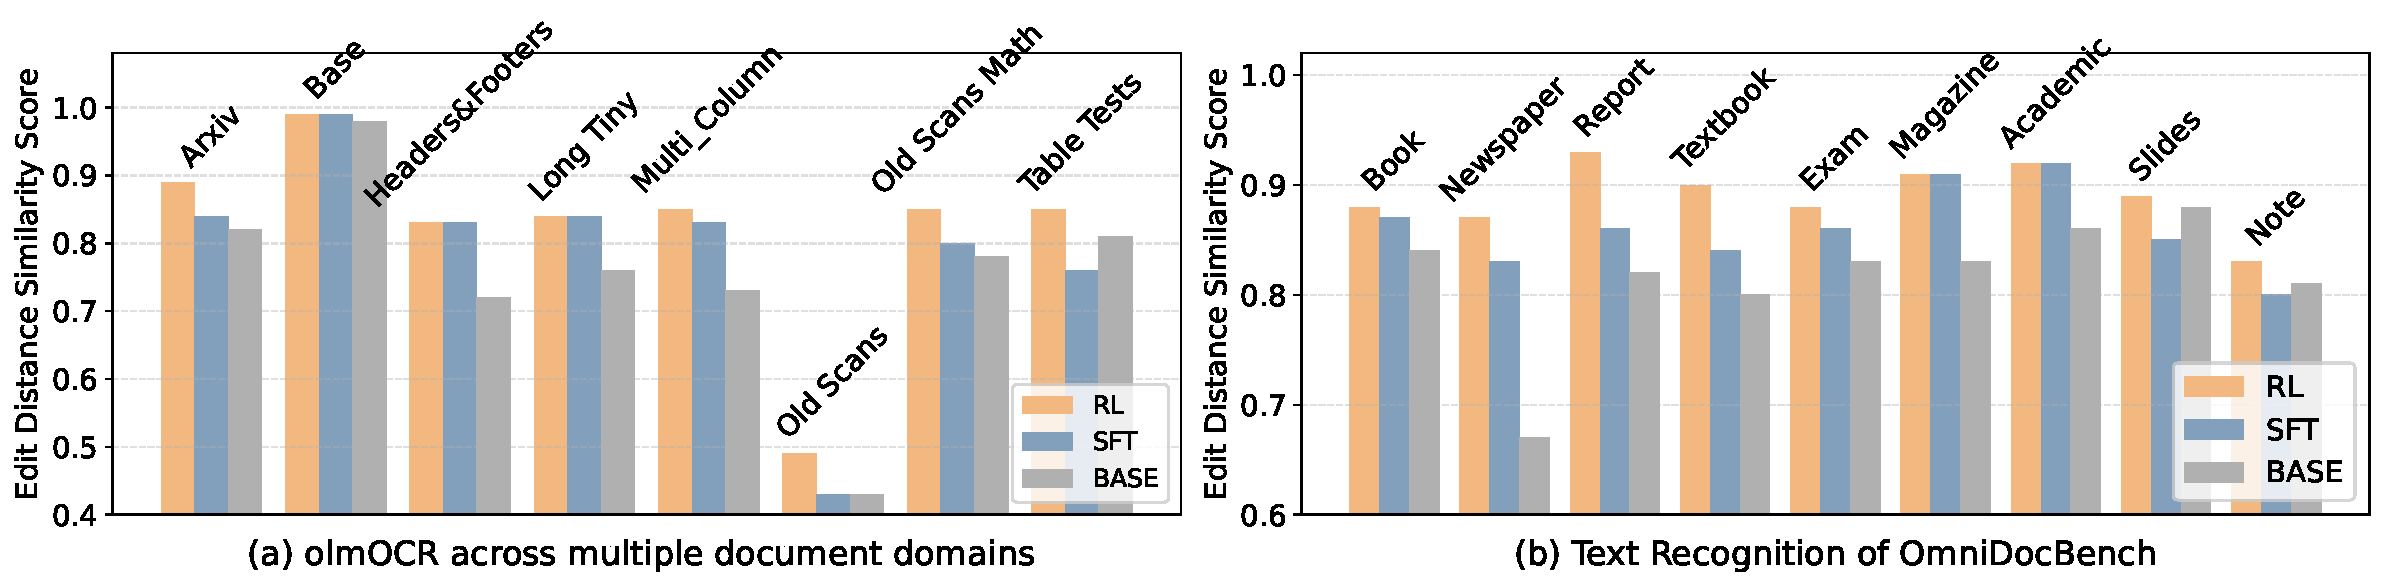
\includegraphics[width=\textwidth]{picture/two_plots_side_by_side_with_names.pdf}
    \vspace{-5mm}
    \caption{Comparison of model performance on different document parsering tasks.}
    \label{fig:olmocr-omnibench}
    \vspace{-3mm}
\end{figure}



\subsection{Further Analysis of LayoutRL}
\label{subsec:further_analysis}

We analyze the behavior of Layout-Aware RL compared with SFT across various document understanding settings. Our analysis focuses on three aspects: training stability, robustness across diverse document types, and generalization under distribution shifts. In particular, the third analysis examines generalization when the training data do not include the textbook and slides domains, which are used only for evaluation. This setup naturally forms OOD scenarios, allowing us to assess how well each model generalizes to unseen document types and layouts.



\paragraph{Training Stability Across Task Types.} As shown in Figure~\ref{fig:metrics_comparison}, we compare SFT and Layout-Aware RL on four OmniDocBench sub-tasks: table recognition, text recognition, formula parsing, and reading order prediction. Across all tasks, RL consistently achieves better performance, yielding higher scores on TEDS and lower errors on NED. More importantly, the RL curves exhibit smoother trajectories with stable improvements over training, while SFT shows large fluctuations and even performance regressions at certain stages. These results indicate that layout-aware rewards not only improve final accuracy but also enhance training stability throughout optimization.




\begin{figure}[t!]
    \centering
    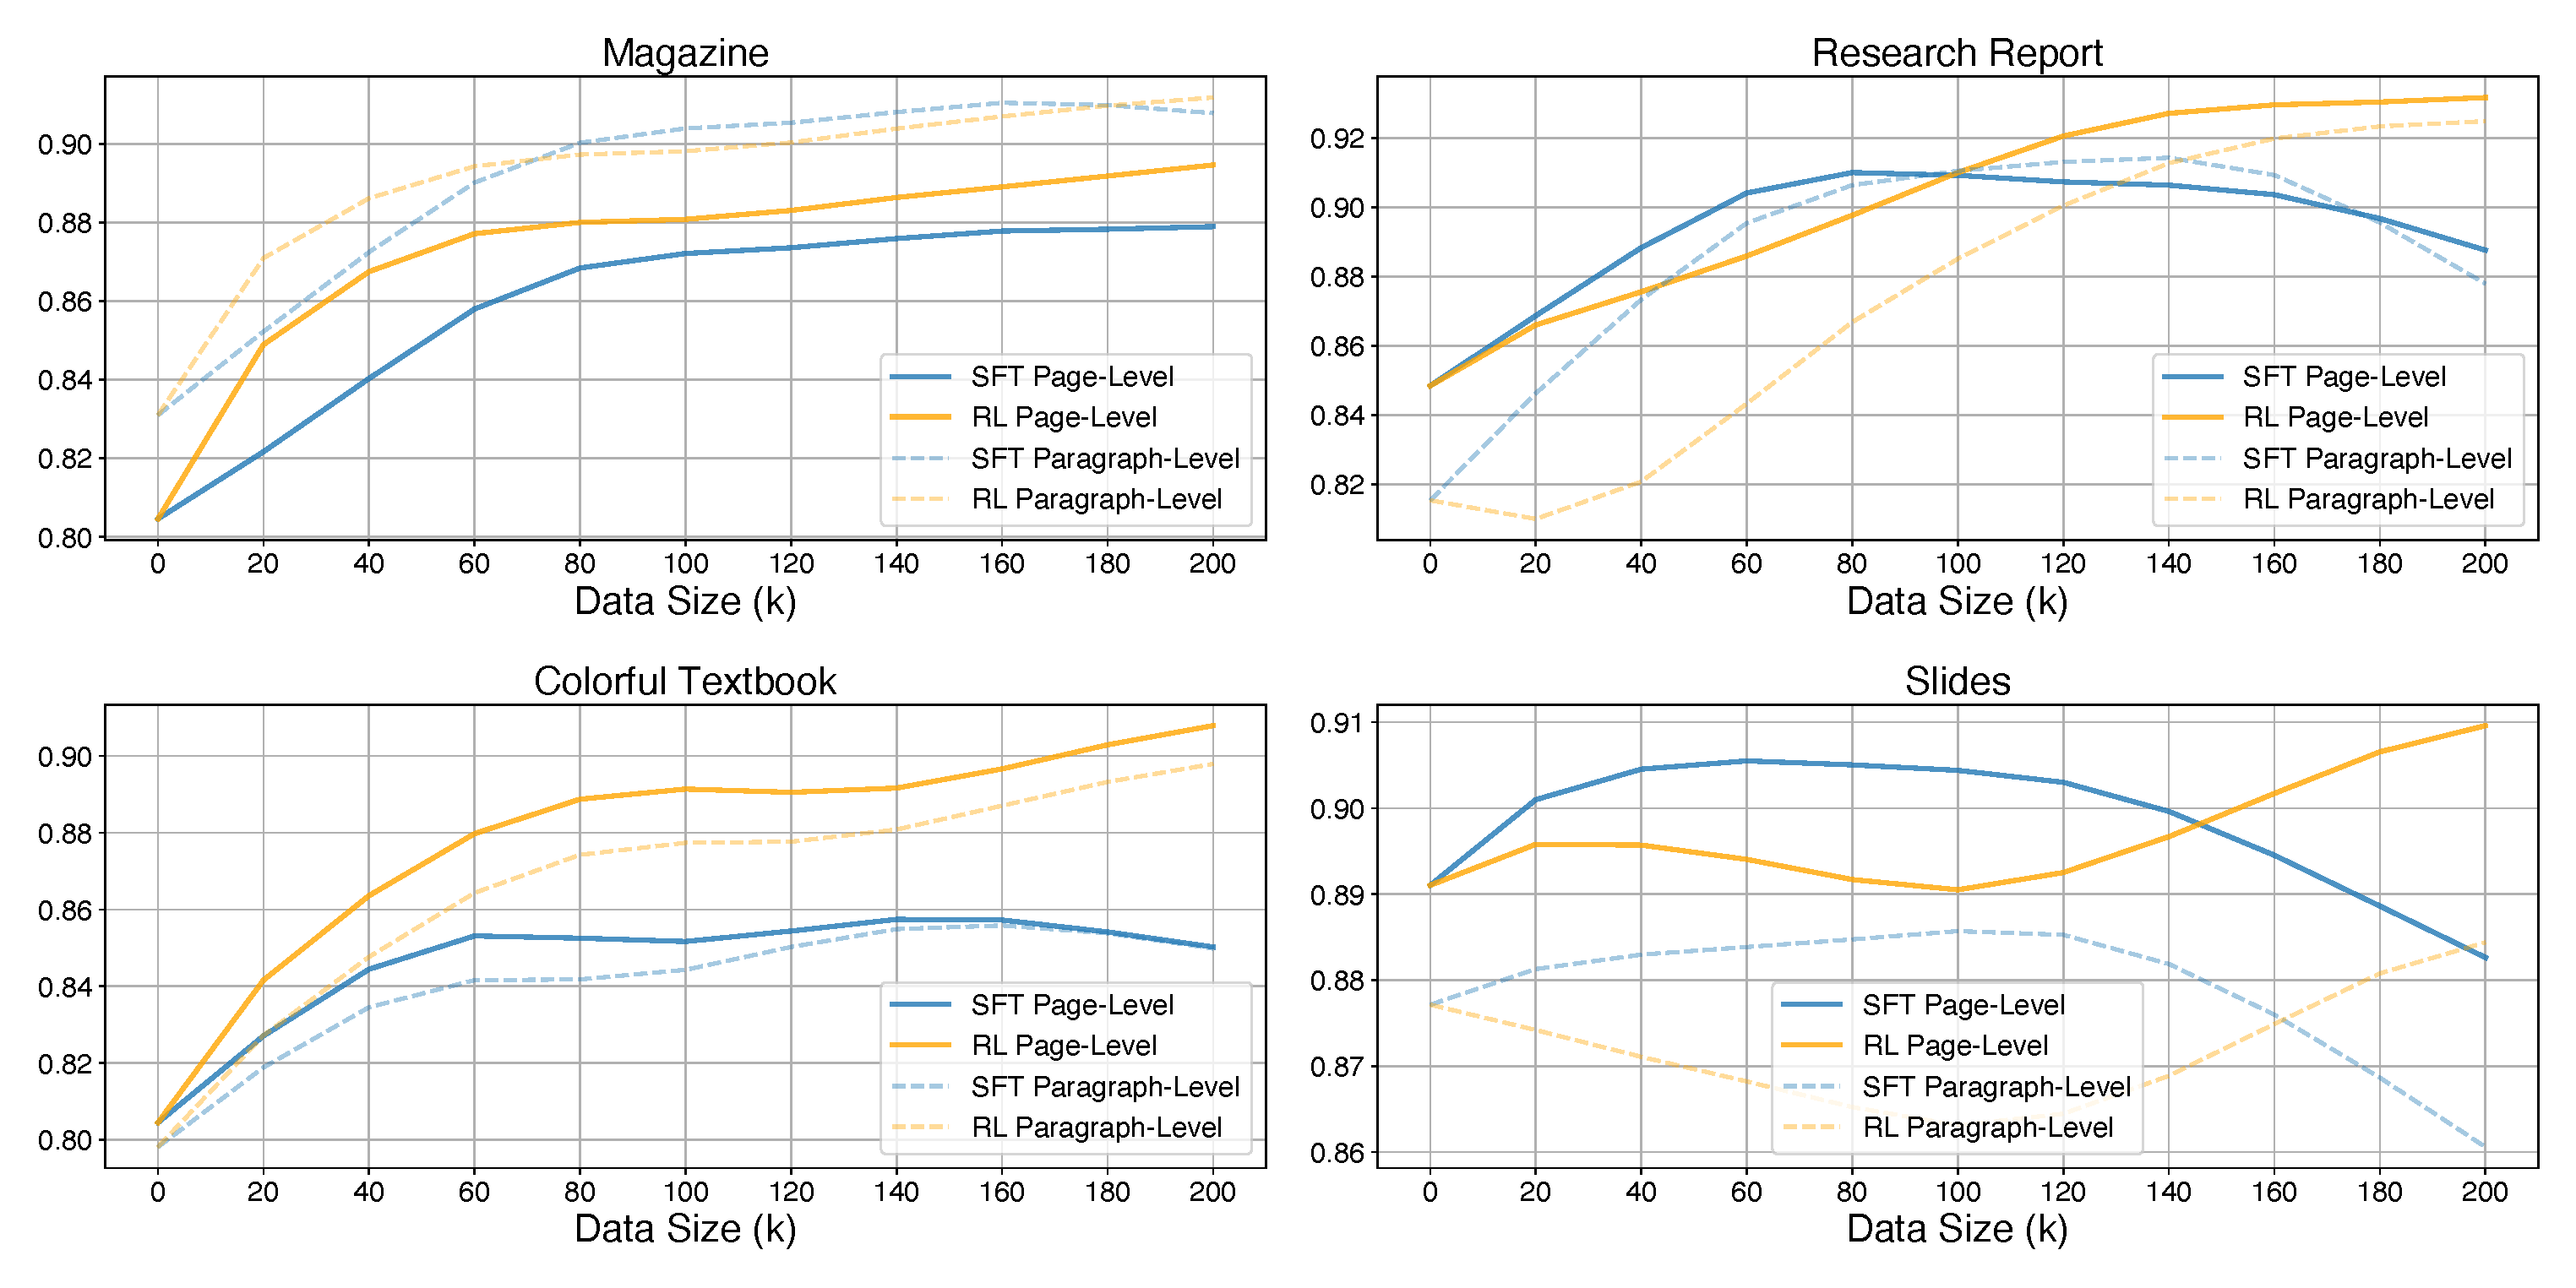
\includegraphics[width=\textwidth]{picture/Four_Figure_Panel_2x2_VECTOR.pdf}
    \vspace{-2mm}
    \caption{Generalization comparison of SFT and Layout-Aware RL. X-axis represents training steps. Y-axis represents 1-NED scores.}
    \label{fig:olmocr-omnibench222}
    \vspace{-3mm}
\end{figure}


\paragraph{Robustness Across Diverse Document Tasks.} Figure~\ref{fig:olmocr-omnibench} compares RL, SFT, and Zero-Shot (Base) across diverse document parsing tasks. On olmOCR (left), RL consistently achieves higher Levenshtein distance similarity score, especially on challenging cases like old scans and table tasks. At the same time, SFT offers moderate gains over Zero-Shot but remains behind RL. On OmniDocBench (right), RL also outperforms the other methods across most document types, showing notable improvements on books, reports, and academic texts. Overall, RL demonstrates greater robustness and better generalization in both structural parsing on olmOCR and text recognition on omnidocbench.





% \begin{figure}[ht]
%     \centering
%     \includegraphics[width=\textwidth]{picture/all_trend2.pdf}
%     \vspace{-2mm}
%     \caption{Generalization comparison of SFT and Layout-Aware RL. X-axis represents training steps. Y-axis represents 1-NED scores.}
%     \label{fig:olmocr-omnibench222}
%     \vspace{-3mm}
% \end{figure}




\paragraph{Analysis of Generalization} 
The Figure~\ref{fig:olmocr-omnibench222} compares document parsing performance across different training steps. The top two plots (magazine, research report) correspond to In-Distribution settings, where training and evaluation domains are aligned, while the bottom two plots (colorful textbook, slides) correspond to OOD settings, where evaluation involves unseen document types. In the in-distribution case, SFT achieves stable paragraph-level accuracy but its page-level performance tends to plateau, reflecting reliance on surface patterns. By contrast, RL continues to improve with data scale, achieving notable gains in page-level accuracy. In the OOD case, SFT performance degrades more severely, while RL maintains robustness and shows stronger improvements, highlighting its ability to capture global structural dependencies and generalize across distributions.




% \begin{table}[h!]
% \centering
% \small
% \begin{tabular}{ccccc}
% \toprule
% Model & AI2D & TextVQA & DocVQA & InfoVQA \\
% \midrule
% Zero-Shot & 82.38 & 82.53 & 94.72 & 81.70 \\
% SFT  & 82.93 (\textcolor{red}{+0.55}) & 80.83 (\textcolor{blue}{-1.70}) & 93.45 (\textcolor{blue}{-1.27}) & 80.14 (\textcolor{blue}{-1.56}) \\
% RL   & 83.13 (\textcolor{red}{+0.75}) & 83.27 (\textcolor{red}{+0.74}) & 95.30 (\textcolor{red}{+0.58}) & 81.81 (\textcolor{red}{+0.11}) \\
% \bottomrule
% \end{tabular}
% \caption{Performance comparison with relative improvements over Zero-Shot. }
% \label{tab:qa_results}
% \vspace{-5mm}
% \end{table}



% \paragraph{Cross-task Transferability.} Interestingly, after large-scale scanned document parsing training, we observe clear divergences in cross-task transfer between RL and SFT. As shown in Table~\ref{tab:qa_results}, RL consistently improves performance on downstream VQA tasks~\citep{kembhavi2016diagram,singh2019towards,mathew2021docvqa,mathew2022infographicvqa}. This indicates that reward-driven optimization enables models to acquire transferable document parsing rules, such as enforcing global structural consistency and text–region grounding, which can even generalize to document question answering tasks with similar data characteristics. In contrast, SFT shows degraded performance relative to the base model, as strict token-level supervision tends to overfit source-format statistics and overwrite previously useful knowledge, leading to negative transfer and a form of distributional forgetting. These findings highlight the superiority of RL in promoting both robust cross-task generalization and knowledge retention.


% % (AI2D~\citep{kembhavi2016diagram}, TextVQA~\citep{singh2019towards}, DocVQA~\citep{mathew2021docvqa}, and InfoVQA~\citep{mathew2022infographicvqa})

 
